%% Run LaTeX on this file several times to get Table of Contents,
%% cross-references, and citations.

\documentclass[11pt]{book}
\usepackage{gvv}
\usepackage{gvv-book-bkup}
%\usepackage{Wiley-AuthoringTemplate}
\usepackage[sectionbib,authoryear]{natbib}% for name-date citation comment the below line
%\usepackage[sectionbib,numbers]{natbib}% for numbered citation comment the above line

%%********************************************************************%%
%%       How many levels of section head would you like numbered?     %%
%% 0= no section numbers, 1= section, 2= subsection, 3= subsubsection %%
\setcounter{secnumdepth}{3}
%%********************************************************************%%
%%**********************************************************************%%
%%     How many levels of section head would you like to appear in the  %%
%%				Table of Contents?			%%
%% 0= chapter, 1= section, 2= subsection, 3= subsubsection titles.	%%
\setcounter{tocdepth}{2}
%%**********************************************************************%%
\setcounter{tocdepth}{3}
%\includeonly{ch01}
\makeindex

\begin{document}

\frontmatter
%%%%%%%%%%%%%%%%%%%%%%%%%%%%%%%%%%%%%%%%%%%%%%%%%%%%%%%%%%%%%%%%
%% Title Pages
%% Wiley will provide title and copyright page, but you can make
%% your own titlepages if you'd like anyway
%% Setting up title pages, type in the appropriate names here:

\booktitle{CBSE Math}

\subtitle{Made Simple}

\AuAff{G. V. V. Sharma}

%% \\ will start a new line.
%% You may add \affil{} for affiliation, ie,
%\authors{Robert M. Groves\\
%\affil{Universitat de les Illes Balears}
%Floyd J. Fowler, Jr.\\
%\affil{University of New Mexico}
%}

%% Print Half Title and Title Page:
%\halftitlepage
\titlepage

%%%%%%%%%%%%%%%%%%%%%%%%%%%%%%%%%%%%%%%%%%%%%%%%%%%%%%%%%%%%%%%%
%%Copyright Page

\begin{copyrightpage}{2023}
%Title, etc
\end{copyrightpage}

% Note, you must use \ to start indented lines, ie,
% 
% \begin{copyrightpage}{2004}
% Survey Methodology / Robert M. Groves . . . [et al.].
% \       p. cm.---(Wiley series in survey methodology)
% \    ``Wiley-Interscience."
% \    Includes bibliographical references and index.
% \    ISBN 0-471-48348-6 (pbk.)
% \    1. Surveys---Methodology.  2. Social 
% \  sciences---Research---Statistical methods.  I. Groves, Robert M.  II. %
% Series.\\

% HA31.2.S873 2004
% 001.4'33---dc22                                             2004044064
% \end{copyrightpage}

%%%%%%%%%%%%%%%%%%%%%%%%%%%%%%%%%%%%%%%%%%%%%%%%%%%%%%%%%%%%%%%%
%% Only Dedication (optional) 

%\dedication{To my parents}

\tableofcontents

%\listoffigures %optional
%\listoftables  %optional

%% or Contributor Page for edited books
%% before \tableofcontents

%%%%%%%%%%%%%%%%%%%%%%%%%%%%%%%%%%%%%%%%%%%%%%%%%%%%%%%%%%%%%%%%
%  Contributors Page for Edited Book
%%%%%%%%%%%%%%%%%%%%%%%%%%%%%%%%%%%%%%%%%%%%%%%%%%%%%%%%%%%%%%%%

% If your book has chapters written by different authors,
% you'll need a Contributors page.

% Use \begin{contributors}...\end{contributors} and
% then enter each author with the \name{} command, followed
% by the affiliation information.

% \begin{contributors}
% \name{Masayki Abe,} Fujitsu Laboratories Ltd., Fujitsu Limited, Atsugi, Japan
%
% \name{L. A. Akers,} Center for Solid State Electronics Research, Arizona State University, Tempe, Arizona
%
% \name{G. H. Bernstein,} Department of Electrical and Computer Engineering, University of Notre Dame, Notre Dame, South Bend, Indiana; formerly of
% Center for Solid State Electronics Research, Arizona
% State University, Tempe, Arizona 
% \end{contributors}

%%%%%%%%%%%%%%%%%%%%%%%%%%%%%%%%%%%%%%%%%%%%%%%%%%%%%%%%%%%%%%%%
% Optional Foreword:

%\begin{foreword}
%\lipsum[1-2]
%\end{foreword}

%%%%%%%%%%%%%%%%%%%%%%%%%%%%%%%%%%%%%%%%%%%%%%%%%%%%%%%%%%%%%%%%
% Optional Preface:

%\begin{preface}
%\lipsum[1-1]
%\prefaceauthor{}
%\where{place\\
% date}
%\end{preface}

% ie,
% \begin{preface}
% This is an example preface.
% \prefaceauthor{R. K. Watts}
% \where{Durham, North Carolina\\
% September, 2004}

%%%%%%%%%%%%%%%%%%%%%%%%%%%%%%%%%%%%%%%%%%%%%%%%%%%%%%%%%%%%%%%%
% Optional Acknowledgments:

%\acknowledgments
%\lipsum[1-2]
%\authorinitials{I. R. S.}  

%%%%%%%%%%%%%%%%%%%%%%%%%%%%%%%%
%% Glossary Type of Environment:

% \begin{glossary}
% \term{<term>}{<description>}
% \end{glossary}

%%%%%%%%%%%%%%%%%%%%%%%%%%%%%%%%
%\begin{acronyms}
%\acro{ASTA}{Arrivals See Time Averages}
%\acro{BHCA}{Busy Hour Call Attempts}
%\acro{BR}{Bandwidth Reservation}
%\acro{b.u.}{bandwidth unit(s)}
%\acro{CAC}{Call / Connection Admission Control}
%\acro{CBP}{Call Blocking Probability(-ies)}
%\acro{CCS}{Centum Call Seconds}
%\acro{CDTM}{Connection Dependent Threshold Model}
%\acro{CS}{Complete Sharing}
%\acro{DiffServ}{Differentiated Services}
%\acro{EMLM}{Erlang Multirate Loss Model}
%\acro{erl}{The Erlang unit of traffic-load}
%\acro{FIFO}{First in - First out}
%\acro{GB}{Global balance}
%\acro{GoS}{Grade of Service}
%\acro{ICT}{Information and Communication Technology}
%\acro{IntServ}{Integrated Services}
%\acro{IP}{Internet Protocol}
%\acro{ITU-T}{International Telecommunication Unit -- Standardization sector}
%\acro{LB}{Local balance}
%\acro{LHS}{Left hand side}
%\acro{LIFO}{Last in - First out}
%\acro{MMPP}{Markov Modulated Poisson Process}
%\acro{MPLS}{Multiple Protocol Labeling Switching}
%\acro{MRM}{Multi-Retry Model}
%\acro{MTM}{Multi-Threshold Model}
%\acro{PASTA}{Poisson Arrivals See Time Averages}
%\acro{PDF}{Probability Distribution Function}
%\acro{pdf}{probability density function}
%\acro{PFS}{Product Form Solution}
%\acro{QoS}{Quality of Service}
%\acro{r.v.}{random variable(s)}
%\acro{RED}{random early detection}
%\acro{RHS}{Right hand side}
%\acro{RLA}{Reduced Load Approximation}
%\acro{SIRO}{service in random order}
%\acro{SRM}{Single-Retry Model}
%\acro{STM}{Single-Threshold Model}
%\acro{TCP}{Transport Control Protocol}
%\acro{TH}{Threshold(s)}
%\acro{UDP}{User Datagram Protocol}
%\end{acronyms}

\setcounter{page}{1}

\begin{introduction}
This book links high school coordinate geometry to linear algebra and matrix analysis through solved problems.

\end{introduction}

\mainmatter

\chapter{Vectors}
\section{2024}
\subsection{12}
%\begin{document}

\begin{center}
     \section*{vectors}   
\end{center}
\begin{enumerate}
\item \textbf{Assertion (A): } The vectors
	\begin{align*}
 \vec{a} = 6\hat{i}+2\hat{j}-8\hat{k}\\
 \vec{b} = 10\hat{i}-2\hat{j}-6\hat{k}\\
 \vec{c} = 4\hat{i}-4\hat{j}+2\hat{k}
	\end{align*}
 \centerline{represent the sides of a right angled triangle.}

 \textbf{Reason (R): } Three non-zero vectors of which none of two are collinear form a triangle if their resultant is zero vector or sum of any two vectors is equal to the third.
\item Find the vector equation of the line passing through the point (2, 3, -5) and making equal angles with the coordinate axes.
\item $\text{Find the projection of vector }(\vec{b} + \vec{c}) \text{ on vector } \vec{a}, \text{ where } \vec{a} = 2\hat{i} + 2\hat{j} + \hat{k}, \vec{b} = \hat{i} + 3\hat{j} + \hat{k}, \text{ and } \vec{c} = \hat{i} + \hat{k}.$
\item  Find the coordinates of the foot of the perpendicular drawn from the point $(2, 3, -8)$ to the line $\frac{4-x}{2} = \frac{y}{6} = \frac{1-z}{3}$.

Also, find the perpendicular distance of the given point from the line.
\item \text{Find the shortest distance between the lines } $L_1$  \& $ L_2$ \text{ given below:}
$L_1$: \text{ The line passing through }(2,-1, 1) \text{ and parallel to }$ \frac{x}{1} = \frac{y}{1} = \frac{z}{3}$\\
$L_2$: $\vec{r} = \hat{i} + (2\mu+1)\hat{j} - (\mu+2)\hat{k}.$

\end{enumerate}


%\begin{document}

%\begin{center}
 %    \section*{vectors}   
%\end{center}
\begin{enumerate}
\item \textbf{Assertion (A): } The vectors
	\begin{align*}
 \vec{a} = 6\hat{i}+2\hat{j}-8\hat{k}\\
 \vec{b} = 10\hat{i}-2\hat{j}-6\hat{k}\\
 \vec{c} = 4\hat{i}-4\hat{j}+2\hat{k}
	\end{align*}
 \centerline{represent the sides of a right angled triangle.}

 \textbf{Reason (R): } Three non-zero vectors of which none of two are collinear form a triangle if their resultant is zero vector or sum of any two vectors is equal to the third.
\item Find the vector equation of the line passing through the point (2, 3, -5) and making equal angles with the coordinate axes.
\item $\text{Find the projection of vector }(\vec{b} + \vec{c}) \text{ on vector } \vec{a}, \text{ where } \vec{a} = 2\hat{i} + 2\hat{j} + \hat{k}, \vec{b} = \hat{i} + 3\hat{j} + \hat{k}, \text{ and } \vec{c} = \hat{i} + \hat{k}.$
\item  Find the coordinates of the foot of the perpendicular drawn from the point $(2, 3, -8)$ to the line $\frac{4-x}{2} = \frac{y}{6} = \frac{1-z}{3}$.

Also, find the perpendicular distance of the given point from the line.
\item \text{Find the shortest distance between the lines } $L_1$  \& $ L_2$ \text{ given below:}
$L_1$: \text{ The line passing through }(2,-1, 1) \text{ and parallel to }$ \frac{x}{1} = \frac{y}{1} = \frac{z}{3}$\\
$L_2$: $\vec{r} = \hat{i} + (2\mu+1)\hat{j} - (\mu+2)\hat{k}.$

\end{enumerate}


\begin{document}

\begin{center}
     \section*{vectors}   
\end{center}
\begin{enumerate}
\item \textbf{Assertion (A): } The vectors
	\begin{align*}
 \vec{a} = 6\hat{i}+2\hat{j}-8\hat{k}\\
 \vec{b} = 10\hat{i}-2\hat{j}-6\hat{k}\\
 \vec{c} = 4\hat{i}-4\hat{j}+2\hat{k}
	\end{align*}
 \centerline{represent the sides of a right angled triangle.}

 \textbf{Reason (R): } Three non-zero vectors of which none of two are collinear form a triangle if their resultant is zero vector or sum of any two vectors is equal to the third.
\item Find the vector equation of the line passing through the point (2, 3, -5) and making equal angles with the coordinate axes.
\item $\text{Find the projection of vector }(\vec{b} + \vec{c}) \text{ on vector } \vec{a}, \text{ where } \vec{a} = 2\hat{i} + 2\hat{j} + \hat{k}, \vec{b} = \hat{i} + 3\hat{j} + \hat{k}, \text{ and } \vec{c} = \hat{i} + \hat{k}.$
\item  Find the coordinates of the foot of the perpendicular drawn from the point $(2, 3, -8)$ to the line $\frac{4-x}{2} = \frac{y}{6} = \frac{1-z}{3}$.

Also, find the perpendicular distance of the given point from the line.
\item \text{Find the shortest distance between the lines } $L_1$  \& $ L_2$ \text{ given below:}
$L_1$: \text{ The line passing through }(2,-1, 1) \text{ and parallel to }$ \frac{x}{1} = \frac{y}{1} = \frac{z}{3}$\\
$L_2$: $\vec{r} = \hat{i} + (2\mu+1)\hat{j} - (\mu+2)\hat{k}.$

\end{enumerate}


%\section{2020}
%\subsection{10}
%\input{2020/vetors1.0.tex}
%\subsection{12}
%\input{2020/vetors2.0.tex}



\chapter{Linear Forms}
%\section{2023}
%\subsection{10}
\section{2024}
\subsection{12}
\begin{enumerate}


\item Students of a school are taken to a railway museum to learn about railways heritage and its history\\
	\begin{figure}[h!]
		\centering
		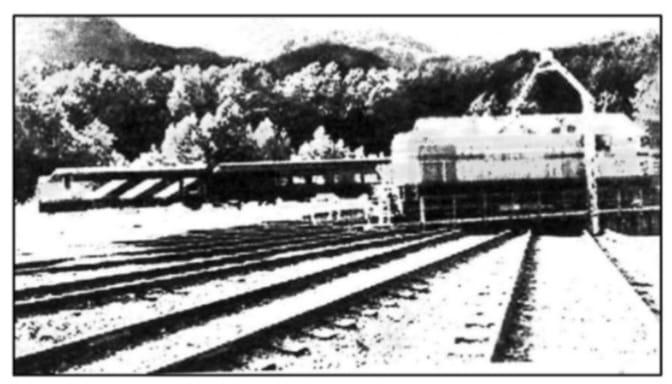
\includegraphics[width=0.8\textwidth]{figs/fig1.jpg}
		\label{fig:image1}
	\end{figure}
	An exhibt in the museum depicted many rail lines on the tack near the railway station. let $L$ be the set of all ral lines on the railwa track and $R$ be the relation on $L$ defined by\\
		$R$={$(l_{1},l_{2}):l_{1} $is parallel to $l_{2}$}\\
	On the basis of the above information, answer the following questions:
\begin{enumerate}
\item Find whether the relation $R$ is symmetric or not.

\item Find whether the relation $R$ is transitive or not.

\item If one of the rail lines on the railway track is represented by the equation $y = 3x + 2$ then find the set of rail lines in $R$ related to it.

\end{enumerate}
\item Let $S$ be the relation defined by $S$ = {$( l_{1},l_{2}):l_{1}$ is perpendicular to $l_{2}$} check whether the relation $S$ is symmetric and transitive.



\end{enumerate}


%\input{2023/linear-10th.tex}
%\subsection{12}                                                                                                  
%\input{2023/linear-12th.tex}
%\section{2022}

\chapter{Circles}

%\section{2010}
%\subsection{12}
%\input{2010/circles.tex}


\chapter{Intersection of Conics}

%\section{2010}
%\subsection{12}
%\input{2010/intersec.tex}





\chapter{Probability}
\section{2024}
\subsection{12}
\input{2024/probability.tex}
\begin{enumerate}
\item An urn contains 3 red and 2 white marbles. Two marbles are drawn one by one with replacement from the urn. Find the probability distribution of the number of white balls. Also, find the mean of the number of white balls drawn.
\item A departmental store sends bills to charge its customers once a month Past experience shows that $ 70\% $ of its customers pay their first month bill in time. The store also found that the customer who pays the bill in time has the probability of 0.8 of paying in time next month and the customer who doesn't pay in time has the probability of 0.4 of paying in time the next month.

Based on the above information, answer the following question:
\begin{enumerate}
\item Let  $E_1$ and $E_2$ respectively denote the event of customer paying or not paying the first month bill in time\\
Find $P(E_1),P(E_2).$
\item Let A denotes the event of customer paving some month's bill in time, then find $P(A|E_1)$ and $P(A|E_2).$
\item Find the probability of customer paying second month's bill in time.
\end{enumerate}

\item Find the probability of customer paying first month's bill in time if it is found that customer has paid the second month's bill in time
%\end{enumerate}


\item Bag I contains 3 red and black balls, Bag II contains 5 red and 2 black balls. Two balls are transferred at random from Bag I to Bag II and then a ball is drawn at random from Bag II. Find the probability that the drawn ball is red in colour.
% \item A departmental store sends bills to charge its customers once a month. Past experience shows that 70\% of its customers pay their first month bill in time. The store also found that the customer who pays the bill in time has the probability of 0.8 of paying in time next month and the customer who doesn't pay in time has the probability of 0.4 of paying in time the next month.
% Based on the above information, answer the following questions:		
% \begin{enumerate}
%	\item[(i)] Let $E_{1}$ and $E_{2}$ respectively denote the event of customer paying or not paying the first month bill in time.\\ Find $P(E_{1})$,$P(E_{2})$
%	\item[(ii)] Let A denotes the event of customer paying second month's bill in time, then find $P( A|E_{1} ) and P( A |E_{2})$.
%	\item[(iii)] Find the probability of customer paying second month's bill in time.
%	\item[(iv)] Find the probability of customer paying first month's bill in time if it is found that customer has paid the second month's bill in time.
%\end{enumerate}


\end{enumerate}


\subsection{10}

\begin{enumerate}

\item If the probability of a player winning a game is 0.79, then the probability of his losing the same game is:
\begin{enumerate}    
    \item $1.79$
    \item $0.31$
    \item $0.21	$                                                           
    \item $0.21$
\end{enumerate}

\item From the data $1, 4, 7, 9, 16, 21, 25$, if all the even numbers are removed, then the probability of getting at random a prime number from the remaining is:
	\begin{enumerate}
\item $\frac{2}{5}$
    \item $\frac{1}{5}$
    \item $\frac{1}{7}$
    \item $\frac{2}{7}$
	\end{enumerate}

\item For some data $x_{1}, x_{2}, \dots, x_{n}$ with respective frequencies $f_{1}, f_{2}, \dots, f_{n}$, the value of $\sum_{i}^{n}f_{i} \brak{x_{i} - \overline{x}}$ is equal to:
	\begin{enumerate}    
\item $n \overline{x}$
    \item $1$
    \item $\Sigma f_{i}$
    \item $0$
	\end{enumerate}

\item The middle-most observation of every data arranged in order is called:
	\begin{enumerate}    
\item mode
    \item median
    \item mean
    \item deviation
\end{enumerate}
\newpage
\item Two dice are rolled together. The probability of getting a sum of numbers on the two dice as $2$, $3$, or $5$ is:
	\begin{enumerate}    
\item $\frac{7}{36}$
    \item $\frac{11}{36}$
    \item $\frac{5}{36}$
    \item $\frac{4}{9}$
	\end{enumerate}
\end{enumerate}

\section{2023}
\subsection{10}
\begin{enumerate}
\item A student noted the number of cars passing through a spot on a road for $100$ periods each of $3$ minutes and summarised it in the table given below. Find the mean and median of the following data.\\

	\begin{tabular}{|c|c|c|c|c|c|c|c|c|}
\hline
Number of cars & 0-10 & 10-20 & 20-30 & 30-40 & 40-50 & 50-60 & 60-70 & 70-80\\ 
\hline
Frequency (Periods) & 7 & 14 & 13 & 12 & 20 & 11 & 15 & 8\\ 
\hline

\end{tabular}

\item Computer-based learning $\brak{CBL}$ refers to any teaching methodology that makes use of computers for information transmission. At an elementary school level, computer applications can be used to display multimedia lesson plans. A survey was done on $1000$ elementary and secondary schools of Assam and they were classified by the number of computers they had.

	\begin{figure}[!ht]
		\centering
		\includegraphics[width=\columnwidth]{figs/last1.jpg}
		\caption{}
		\label{fig:enter-label}
	\end{figure}

	\begin{center}
	\begin{tabular}{|c|c|c|c|c|c|}
	\hline
	\textbf{Number of computers} & 1-10 & 11-20 & 21-50 &  51-100 & 101 and more \\
	\hline
	\textbf{Number of Schools} & 250 & 200 & 290 & 180 & 80 \\
	\hline
	\end{tabular}
	\end{center}

	\text One school is chosen at random.Then:
	\begin{enumerate}
		\item  Find the probability that the school chosen at random has more than $100$ computers.
		\item
		\begin{enumerate}
			\item  Find the probability that the school chosen at random has $50$ or fewer computers.
			\item  Find the probability that the school chosen at random has no more than $20$ computers.
		\end{enumerate}
		\item  Find the probability that the school chosen at random has $10$ or less than $10$ computers.
	\end{enumerate}

\item For the following distribution:

\begin{center}
\begin{tabular}{|c|c|c|c|c|c|c|}
\hline
\textbf{Marks Below} & 10 & 20 & 30 & 40 & 50 & 60 \\
\hline
\textbf{Number of Students} & 3 & 12 & 27 & 57 & 75 & 80 \\
\hline
\end{tabular}
\end{center}

The modal class is:

\begin{enumerate}
    \item $10-20$
    \item $20-30$
    \item $30-40$
    \item $50-60$
\end{enumerate}
\item  Two dice are thrown together. The probability of getting the difference of numbers on their upper faces equal to 3 is:

	\begin{enumerate}
	\item  $\frac{1}{9}$
	\item $\frac{2}{9}$
	\item  $\frac{1}{6}$
	\item  $\frac{1}{12}$
\end{enumerate}
\item A Card is drawn at random from a well-shuffled pack of 52 cards.The probability that the card drawn is not an ace is:
\begin{enumerate}
	\item $\frac{1}{13}$
	\item  $\frac{9}{13}$
	\item $\frac{4}{13}$
	\item $\frac{12}{13}$
\end{enumerate}
\item{DIRECTIONS:} In questions number 19 and 20, a statement of Assertion (A) is followed by a statement of Reason (R). Choose the correct option out of the following:
Assertion (A): The probability that a leap year has 53 Sundays is $\frac{2}{7}$.

Reason (R): The probability that a non-leap year has 53 Sundays is $\frac{5}{7}$.

\begin{enumerate}
    \item Both Assertion (A) and Reason (R) are true and Reason (R) is the correct explanation of Assertion (A).
    \item Both Assertion (A) and Reason (R) are true and Reason (R) is not the correct explanation of Assertion (A).
    \item Assertion (A) is true but Reason (R) is false.
    \item Assertion (A) is false but Reason (R) is true.
\end{enumerate}
\end{enumerate}

\section{2006}
\subsection{10}
\input{2006/probabilitysai.tex}
%\section{2010}
%\subsection{12}
%\item Bag I contains 3 red and black balls, Bag II contains 5 red and 2 black balls. Two balls are transferred at random from Bag I to Bag II and then a ball is drawn at random from Bag II. Find the probability that the drawn ball is red in colour.
% \item A departmental store sends bills to charge its customers once a month. Past experience shows that 70\% of its customers pay their first month bill in time. The store also found that the customer who pays the bill in time has the probability of 0.8 of paying in time next month and the customer who doesn't pay in time has the probability of 0.4 of paying in time the next month.
% Based on the above information, answer the following questions:		
% \begin{enumerate}
%	\item[(i)] Let $E_{1}$ and $E_{2}$ respectively denote the event of customer paying or not paying the first month bill in time.\\ Find $P(E_{1})$,$P(E_{2})$
%	\item[(ii)] Let A denotes the event of customer paying second month's bill in time, then find $P( A|E_{1} ) and P( A |E_{2})$.
%	\item[(iii)] Find the probability of customer paying second month's bill in time.
%	\item[(iv)] Find the probability of customer paying first month's bill in time if it is found that customer has paid the second month's bill in time.
%\end{enumerate}


\end{enumerate}



\chapter{Construction}

%\section{2010}
%\subsection{12}
%\input{2010/construction.tex}


\chapter{Optimization}

\section{2024}
\subsection{12}
\begin{enumerate}



\item Solve the following Linear Programming problem graphically:\\ Maximise $Z=300x + 600y $\\
	Subject to \begin{align}x + 2y \le 12\\
		2x + y \le 12\\
		x +\frac{5}{4}y \ge 5\\
		x \ge 0 , y \ge 0.\end{align}

\end{enumerate}

%\input{2010/opt.tex}


\chapter{Algebra}
\section{2024}
\subsection{10}

\begin{enumerate}


\item If the sum of zeroes of the polynomial $ p\brak x = 2x^2 - k\sqrt2x+1 $ is${\sqrt2} $,then value of k is:
\begin{enumerate}
    \item $ \sqrt{2} $
    \item $2$
    \item $ 2  \sqrt{2} $
    \item $ \frac{1}{2} $
 \end{enumerate}

\item If the roots of the equation $ax^2 + bx + c = 0$,$a \neq 0$ are real and equal, then which of the following relations is true?
\begin{enumerate}    
    \item $a = \frac{b^2}{c}$
    \item $b^2 = ac$                                                                                    \item $ac = \frac{b^2}{4}$
    \item $c = \frac{b^2}{a}$
\end{enumerate}

\item In an A.P., if the first term $a = 7$, $n$th term $a_{n} = 84$, and the sum of the first $n$ terms $s_{n} = \frac{2093}{2}$, then $n$ is equal to:
\begin{enumerate}
    \item $22$
    \item $24$
    \item $23$
    \item $26$
\end{enumerate}

\item The zeroes of a polynomial $x^2 + px + q$ are twice the zeroes of the polynomial $4x^2 - 5x - 6$. The value of $p$ is:
	\begin{enumerate}   
\item $-\frac{5}{2}$
    \item $\frac{5}{2}$
    \item $-5$
    \item $10$
	\end{enumerate}
\newpage
 \item In the given figure, graphs of two linear equations are shown. The pair of these linear equations is:
\begin{figure}[!ht]
\centering
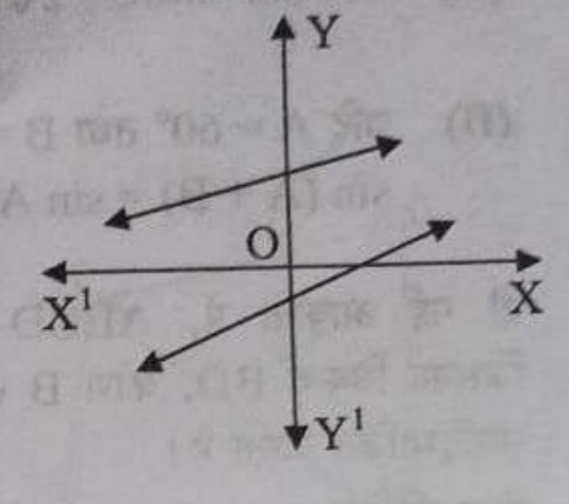
\includegraphics[width=\columnwidth]{figs/Image1.jpg}
\caption{}
\label{fig:enter-label}
\end{figure}
\begin{enumerate}
    \item consistent with a unique solution.
    \item consistent with infinitely many solutions.
    \item inconsistent.
    \item inconsistent but can be made consistent.
\end{enumerate}
\end{enumerate}

\subsection{12}
\input{2024/algebra.tex}
\section{2023}
\subsection{10}
\begin{enumerate}
\item \textbf{Assertion (A):}The polynomial p(x)=$x^{2}+3x+3$ has two real zeroes.
	\\\textbf{Reason (R) :} A quadratic polynomial can have at most two zeroes.
\begin{enumerate}
\item Both Assertion (A) and Reason (R) are true and Reason (R) is the correct explanation of Assertion (A). 
\item Both Assertion (A) and Reason (R) are true and Reason (R) is not the correct explanation of Assertion (A).
\item Assertion (A) is true but Reason (R) is false.
\item Assertion (A) is false but Reason (R) is true.
\end{enumerate}

\item Three bells ring at intervals of $ 6, 12 and 18 minutes$. If all the three bells rang at $ 6 a.m.,$ when will they ring together again ?

\item If the system of linear equations  \\ 		
\begin{align}
		2x + 3y = 7 and \\ 
		2ax + \brak{a+b}y = 28
\end{align}
\text have infinite number of solutions, then find the values of $' a '$and$' b '$.

\item If
\begin{align}
	 217x + 131y = 913 and \\
         131x + 217y = 827,
\end{align}
 then solve the equations for the values of $x$ and $y$.

\item How many terms of the arithmetic progression $45,39,33,......$ must be taken so that their sum is $180$? Explain the double answer.
	 \item The pair of linear equations $2x = 5y + 6$ and $15y = 6x - 18$ represents two lines which are:
    \begin{enumerate}
        \item intersecting
        \item parallel
        \item coincident
        \item either intersecting or parallel
    \end{enumerate}
    \item The next term of the A.P,:$\sqrt 70$,$\sqrt 28$,$\sqrt 63$ is:
	\begin{enumerate}
        \item $\sqrt 70$
	\item $\sqrt 80$
	\item $\sqrt 97$
	\item $\sqrt 112$
\end{enumerate}
\item The roots of the equation $x^2 + 3x - 10 = 0$ are:

\begin{enumerate}
    \item$2, -5$
    \item $-2, 5$
    \item $2, 5$
    \item $-2, -5$
\end{enumerate}
\item If $\alpha, \beta$ are zeroes of the polynomial $x^2 - 1$, then the value of $\brak(\alpha + \beta)$ is:

\begin{enumerate}
    \item $2$
    \item $1$
    \item $-1$
    \item $0$
\end{enumerate}
\item If $ \alpha, \beta $ are the zeroes of the polynomial $ p\brak{x} = 4x^2 - 3x - 7 $, then $ \frac{1}{\alpha} + \frac{1}{\beta} $ is equal to:

\begin{enumerate}
    \item $\frac{7}{3}$
    \item$-\frac{7}{3}$
    \item $\frac{3}{7}$
    \item $-\frac{3}{7}$
\end{enumerate}
\end{enumerate}


\section{2006}                      
\subsection{10}
\input{2006/algebrasai.tex}
%\section{2010}
%\subsection{12}
%\input{2010/algebra.tex}

\chapter{Geometry}
\section{2024}
\subsection{10}

\begin{enumerate}


\item A solid sphere is cut into two hemispheres. The ratio of the surface areas of the sphere to that of the two hemispheres taken together is:
	\begin{enumerate}    
\item $1:1$
    \item $1:4$
    \item $2:3$
    \item $3:2$
	\end{enumerate}

\item The volume of the largest right circular cone that can be carved out from a solid cube of edge $2 \, \text{cm}$ is:
	\begin{enumerate}    
\item $\frac{4\pi}{3} \, \mathrm{cu cm}$
    \item $\frac{5\pi}{3} \, \mathrm{cu cm}$
    \item $\frac{8\pi}{3} \, \mathrm{cu cm}$
    \item $\frac{2\pi}{3} \, \mathrm{cu cm}$
	\end{enumerate}

\item \textbf{Assertion (A):} The tangents drawn at the end points of a diameter of a circle are parallel.

\textbf{Reason (R):} The diameter of a circle is the longest chord.
\begin{enumerate}
    \item Both Assertion (A) and Reason (R) are true, and Reason (R) is the correct explanation of Assertion (A).
    \item Both Assertion (A) and Reason (R) are true, but Reason (R) is not the correct explanation for Assertion (A).
    \item Assertion (A) is true, but Reason (R) is false.
    \item Assertion (A) is false, but Reason (R) is true.
\end{enumerate}

\item $AD$ is a median of $\triangle ABC$ with vertices $A(5, -6)$, $B(6, 4)$, and $C(0, 0)$. The length of $AD$ is equal to:
	\begin{enumerate}    
\item $\sqrt{68}$ units
    \item $2\sqrt{15}$ units
    \item $\sqrt{101}$ units
    \item $10$ units
	\end{enumerate}

 \item If the distance between the points $\brak{3, -5}$ and $\brak{x, -5}$ is 15 units, then the values of $x$ are:
    \begin{enumerate}
    \item $12, -18$
    \item $-12, 18$
    \item $18, 5$
    \item $-9, -12$
    \end{enumerate}

    \item The center of a circle is at $\brak{2, 0}$. If one end of a diameter is at $\brak{6, 0}$, then the other end is at:
	\begin{enumerate}    
		\item $\brak{0, 0}$
		\item $\brak{4, 0}$
		\item $\brak{-2, 0}$
		\item $\brak{-6, 0}$
	\end{enumerate}

\end{enumerate}

\subsection{12}
\begin{enumerate}
	\item The coordinates of the foot of the perpendicular drawn from the point $(0,1,2)$ on th $x$-axis are given by:
		\begin{enumerate}
			\item $(1,0,0)$
			\item $(2,0,0)$
			\item $(\sqrt{5},0,0)$
			\item $(0,0,0)$
		\end{enumerate}
	\item If a line makes an angle of $30^{\circ}$ with the positive direction of $x$-axis, $120^{\circ}$ with the positive direction of $y$-axis, then the angle which it makes with the positive direction of $z$-axis is:
		\begin{enumerate}
			\item $90^{\circ}$
			\item $120^{\circ}$
			\item $60^{\circ}$
			\item $0^{\circ}$
		\end{enumerate}
	\item Find the equation of the line which bisects the line segment joining points $A(2,3,4)$ and $B(4,5,8)$ and is perpendicular to the lines $\frac{x-8}{3} = \frac{y+19}{-16} = \frac{z-10}{7}$ and $\frac{x-15}{3} = \frac{y-29}{8} = \frac{z-5}{-5}$
	\item If $A_{1}$ denotes the area of region bounded by $y^{2} = 4x$ and $x$-axis in the first quadrant and $A_{2}$ denotes the area of region bounded by $y^{2} = 4x$, $x=4$, find $A_{1} : A_{2}$.
%\end{enumerate}


\item Sand is pouring from a pipe at the rate of $ 15 cm^3/minute$. The falling sand forms a cone on the ground such that the height of the cone is always one- third of the radius of the base. How fast is the height of the sand cone increasing at the instant when the height is $4cm$	 


\item A rectangular visiting card is to contain $24 sq.cm.$ of printed matter. The margins at the top and bottom of the card are to be $1 cm$ and the margins on the left and right are to be cm as shown below:

%\newpage
\begin{figure}[h!]
\centering
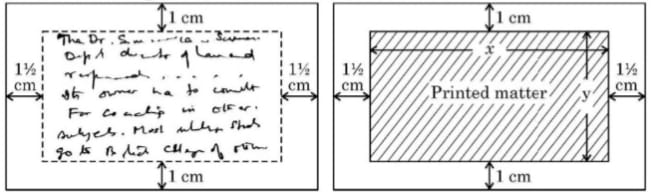
\includegraphics[width=0.8\textwidth]{figs/fig2.jpg}
\label{fig:image2}
\end{figure}

On the basis of the above information, answer the following questions:
\begin{enumerate}
	\item[(i)] Write the expression for the area of the visiting card in terms of x.

	\item[(ii)] Obtain the dimensions of the card of minimum area.



\end{enumerate}


\end{enumerate}

\section{2023}
\subsection{10}
\begin{enumerate}

\item A car has two wipers which do not overlap. Each wiper has a blade of length $21 \mathrm{cm}$ sweeping through an angle of $120\degree$. Find the total area cleaned at each sweep of the two blades.

\item Sides $AB$ and $BC$ and median $AD$ of a triangle $ABC$ are respectively proportional to sides $PQ$ and $QR$ and median $PM$ of $\triangle PQR$.Show that $\triangle ABC \sim \triangle PQR$.

\item Through the mid-point $M$ of the side $CD$ of a parallelogram $ABCD$,the line $BM$ is drawn intersecting $AC$ in $L$ and $AD$ (produced) in $E$.Prove that $EL = 2BL$. 

\item In the given figure, $O$ is the center of the circle .$AB$ and $AC$ are tangents drawn to the circle from point $A$. If $\angle BAC = 65\degree $, then find the measure of $\angle BOC $.
	\begin{figure}[!ht]
		\centering
		\includegraphics[width=\columnwidth]{figs/last5.jpg}
		\caption{}
		\label{fig:enter-label}
	\end{figure}

\newpage
\item In the given figure, $O$ is the centre of the circle and $QPR$ is a tangent to it at $P$.Prove that $\angle QAP + \angle APR = 90\degree$.

	\begin{figure}[!ht]
		\centering
		\includegraphics[width=\columnwidth]{figs/last4.jpg}
		\caption{}
		\label{fig:enter-label}
	\end{figure}
\newpage
\item In an annual day function of a school, the organizers wanted to give a cash prize along with a memento to their best students.Each memento is made as shown in the figure and its base $ABCD$ is shown from the front side.The rate of silver plating \rupee~20 $per  \mathrm{cm}^2$.

	\begin{figure}[!ht]
		\centering
		\includegraphics[width=\columnwidth]{figs/last3.jpg}
		\caption{}
		\label{fig:enter-label}
	\end{figure}

	\text Based on the above, answer the following question:
		\begin{enumerate}
			\item What is the area of the quadrant $ODOC$?
			\item Find the area of $\triangle AOB$.
			\item
			\begin{enumerate}
				\item What is the total cost of silver plating the shaded part $ABCD$?
				\item What is the length of arc $CD$ ?
			\end{enumerate}
		\end{enumerate}
\newpage
\item In a coffee shop, coffee is served in two types of cups.One is cylindrical  in shape with diameter $7 \mathrm{cm}$ and height $14 \mathrm{cm} $ and the other is hemispherical with diameter $21 \mathrm{cm}$.

	
	\begin{figure}[!ht]
		\centering
		\includegraphics[width=\columnwidth]{figs/last2.jpg}
		\caption{}
		\label{fig:enter-label}
	\end{figure}

	\text Based on the above, answer the following question:
	\begin{enumerate}
		\item  Find the area of the cylindrical cup.
		\item
		\begin{enumerate}
			\item  What is the capacity of the hemispherical cup?
			\item Find the capacity of the cylindrical cup.
		\end{enumerate}
		\item   What is the curved surface area of the cylindrical cup?
         \end{enumerate}

\newpage	
\item Show that the points $\brak{-2,3}, \brak{8,3}$ and $\brak{6,7} $ are the vertices of a right-angled triangle.

\item If $Q\brak{0,1}$ is equidistant from $P\brak{5,-3}$ and $R\brak{x,6}$,find the values of $x$.
\item In the given figure, $TA$ is a tangent to the circle with center $O$ such that $OT = 4\mathrm{cm}$, $\angle OTA = 30\degree$, then the length of $TA$ is:
    \begin{enumerate}
        \item $2 \times \sqrt{3} \mathrm{cm}$
        \item $2\mathrm{cm}$
        \item $2 \times \sqrt{2}\mathrm{cm}$
        \item $\sqrt{3}\mathrm{cm}$
    \end{enumerate}
    
\begin{figure}[!ht]
\centering
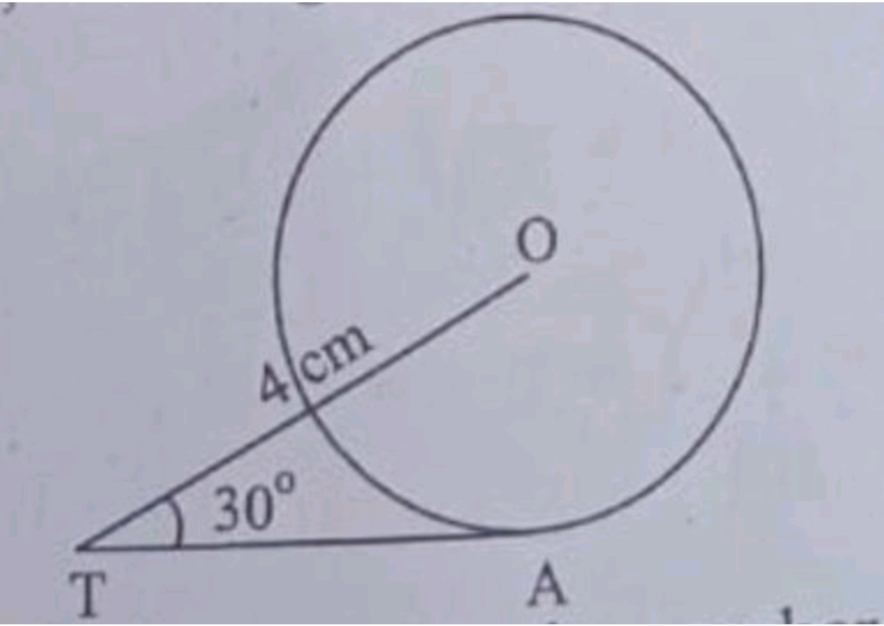
\includegraphics[width=\columnwidth]{figs/image 1.jpg}
\label{fig:image1}
	\caption{image1}
\end{figure}
\item In the given figure,$\triangle ABC \sim \triangle QPR$,If $AC = 6\mathrm{cm},BC = 5 \mathrm{cm},QR = 3\mathrm{cm}  and PR = x$;then the value of  x is:
	\begin{enumerate}
	\item $3.6 \mathrm{cm}$
	\item $2.5\mathrm{cm}$
	\item $10 \mathrm{cm}$
	\item $3.2 \mathrm{cm}$
	\end{enumerate}
	\begin{figure}[!ht]
\centering
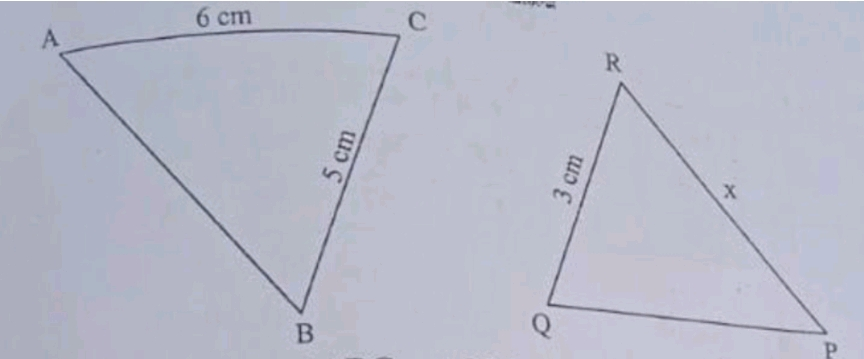
\includegraphics[width=\columnwidth]{figs/image 2.jpg}
\label{fig:image1}
	\caption{image2}
\end{figure}
\item The distance of the point $\brak{-6,8}$ from origin is:
	\begin{enumerate}
	\item $6$
	\item $-6$
	\item $8$
	\item $10$
\end{enumerate}
\item What is the area of a semi-circle of diameter $\brak{d}$?
\begin{enumerate}
    \item $\frac{1}{16} \times \pi \times d^2$
    \item $\frac{1}{4} \times \pi \times d^2$
    \item $\frac{1}{8} \times \pi \times d^2$
    \item $\frac{1}{2} \times \pi \times d^2$
\end{enumerate}
\item In the given figure, $PT$ is a tangent at $T$ to the circle with centre $\brak{o}$. If $\angle TPO = 25\degree$, then $x$ is equal to:
\begin{figure}[!ht]
\centering
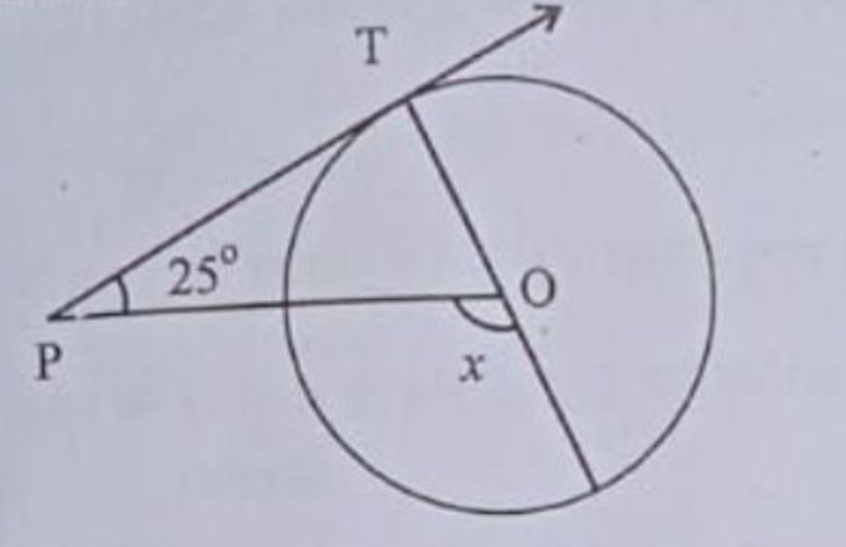
\includegraphics[width=\columnwidth]{figs/image 3.jpg}
\label{fig:image1}
        \caption{image3}
\end{figure}
\begin{enumerate}
    \item $25\degree$
    \item $65\degree$
    \item $90\degree$
    \item $115\degree$
\end{enumerate}
\newpage
\item In the given figure, $PQ \parallel AC$. If $BP = 4 \, \mathrm{cm}$, $AP = 2.4 \mathrm{cm}$, and $BQ = 5 \, \mathrm{cm}$, then the length of $BC$ is:
\begin{figure}[!ht]
\centering
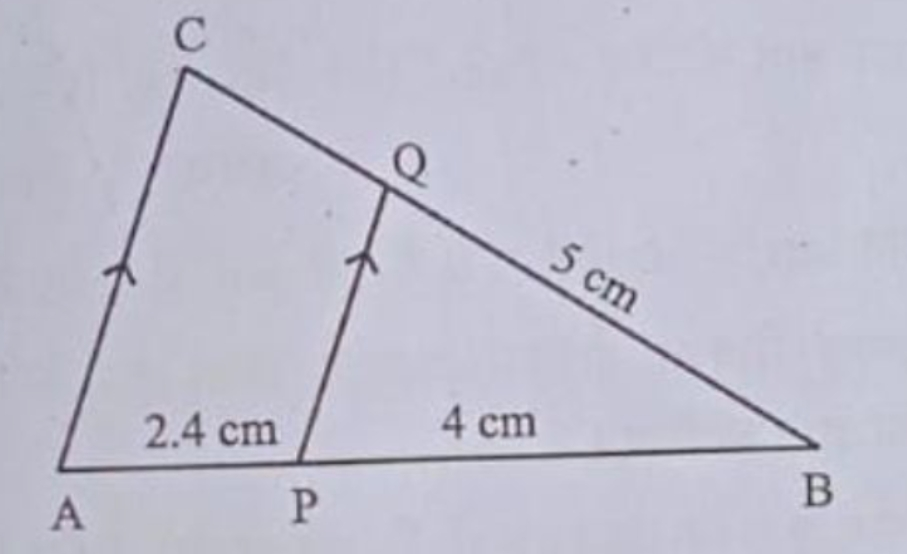
\includegraphics[width=\columnwidth]{figs/image 4.jpg}
\label{fig:image1}                                                  \caption{image4}                                    
\end{figure}
	\begin{enumerate}
    \item $8\mathrm{cm}$
    \item $3\mathrm{cm}$
    \item $0.3 \mathrm{cm}$
    \item $\frac{25}{3}\mathrm{cm}$
\end{enumerate}
\item The points $\brak{-4,0},\brak {4,0}, and \brak{0,3}$ are the vertices of a:

\begin{enumerate}
    \item right triangle
    \item isosceles triangle
    \item equilateral triangle
    \item scalene triangle
\end{enumerate}

\end{enumerate}


\section{2006}
\subsection{10}
\input{2006/geomentrysai.tex}
%\section{2023}
%\subsection{10}
%\input{2023/ASSIGNMENT_1.tex}

\chapter{sequences}
\section{2006}                       
\subsection{10}
\input{2006/sequencesai.tex}

\chapter{Datahandling}
\section{2006}
\subsection{10}
\input{2006/datahandlingsai.tex}

\chapter{Discrete}
%\section{2010}
%\subsection{12}
%\input{2010/discrete.tex}

\chapter{Number Systems}
\section{2024}
\subsection{10}
\begin{enumerate}
\item If two positive integers $p$ and $q$ can be expressed as $p = 18a^2 b^4$ and $q = 20a^3 b^2$ where $a$ and $b$ are prime numbers, then $\text{LCM}(p, q)$ is:
	\begin{enumerate}    
\item $2a^2 b^2$
    \item $180a^2 b^2$
    \item $12a^2  b^2$
    \item $180a^3 b^4$
	\end{enumerate}
\end{enumerate}

\section{2023}
\subsection{10}

\begin{enumerate}

\item Prove that $ 2+\sqrt3 $ is an irrational number,given that $ \sqrt3 $ is an irrational number.

\item Find by prime factorisation the $LCM$ of the number $18180$ and $7575$. Also,find the $HCF$ of the two numbers.

\item The ratio of HCF to LCM of the least composite number and the least prime number is:

	\begin{enumerate}
	\item $1:2$
	\item $2:1$
	\item $1:1$
	\item $1:3$
\end{enumerate}
\end{enumerate}


%\section{2010}
%\subsection{12}
%\input{2010/numbersys.tex}


\chapter{Differentiation}
\section{2024}
\subsection{12}
\input{2024/differetiation.tex}
\begin{enumerate}
	\item The differential equation $\frac{dy}{dx}=F(x,y)$ will not be a homogeneous differential equation, if $F(x,y)$ is:
		\begin{enumerate}
			\item $\cos x - \sin (\frac{y}{x})$
			\item $\frac{y}{x}$
			\item $\frac{x^{2} + y^{2}}{xy}$
			\item $\cos^{2}(\frac{x}{y})$
		\end{enumerate}
	\item The degree of the differential equation $(y'')^{2} + (y')^{3} = x\sin(y')^{3}$ is:
		\begin{enumerate}
			\item $1$
			\item $2$
			\item $3$
			\item not defined
		\end{enumerate}
	\item If $y=\cosec (\cot^{-1} x)$, then prove that $\sqrt{1 + x^{2}} \frac{dy}{dx} -x = 0$.
	\item If $x=e^{\cos 3t}$ and $y=e^{\sin 3t}$, prove that $\frac{dy}{dx} = -\frac{ylogx}{xlogy}$.
	\item Show that: $\frac{d}{dx} (|x|)=\frac{x}{|x|}, x\neq0$.
	\item  Find the particular solution of the differetial equation given by $2xy + y^{2} - 2x^{2} \frac{dy}{dx} = 0; y=2$, when x=1.
	\item Find the general solution of the differential equation:\\
		\centerline {$ydx = (x + 2y^{2})$dy}
%\end{enumerate}

\item Verify whether the function f defined by $f(x) = \begin{cases} x \sin{\left(\frac{1}{x}\right)}, & x \neq 0 \\ 0, & x = 0 \end{cases} $\\
\text{ is continuous at } x = 0 \text{ or not.}


\item Check for differentiability  of the function f defined by $f(x) = |x-5|$, at the point $x = 5$.


\item Find the particular solution of the  differential equation : \\
	$ \frac{dy}{dx} - 2xy = 3x^2e^{x^2} ; y(0)=5 $

\item Solve the following differential equation:\\
	$x^2 dy+y(x+y)dx=0$

\item Find the values of $a$ and $b$ so that the following function is differentiable for all values of $x$  $f(x) = \begin{cases} ax+b, & x>-1 \\ bx^2-3, & x\le -1 \end{cases} $

\item Find $ \frac{dy}{dx},$ if $(\cos{x})^y = (\cos{y})^x.$
\item If $\sqrt{1-x^2} + \sqrt{1-y^2} =a(x-y)$, prove that $ \frac{dy}{dx}= \sqrt{\frac{1-y^2}{1-x^2}}.$



\end{enumerate}


%\section{2023}
%\subsection{12}
%\input{2023/differentiation.tex}






\chapter{Integration}
\section{2024}
\subsection{12}
\begin{enumerate}
	\item $\int\limits_0^{\frac{\pi}{2}} \frac{\sin x - \cos x}{1 + \sin x\cos x}dx$ is equal to:
		 \begin{enumerate}
			 \item $\pi$
			 \item $Zero(0)$
			 \item $\int\limits_0^{\frac{\pi}{2}}$ $\frac{2\sin x}{1+ \sin x\cos x}dx$
			 \item $\frac{\pi^{2}}{4}$
		 \end{enumerate}
	 \item Find : $\int \frac{e^{4x}-1}{e^{4x}+1}dx$
	 \item Evaluate:\\
		 $\int\limits_{2}{-2} \sqrt{\frac{2-x}{z+x}}dx$ 
	 \item Find: \\
		$\int \frac{1}{x[(logx)^{2} - 3logx - 4]}dx$
	\item Find: $\int x^{2} \cdot \sin^{-1} (x^{\frac{3}{2}})dx$ 
%\end{enumerate}

\item Find: $\int \cos^3  x \cdot e^{\log(\sin x)}dx$

\item Find: $\int \frac{1}{5+4x-x^2}dx$	

\item Evaluate: $\int_{0}^{\pi}\frac{e^{\cos{x}}}{e^{\cos{x}} + e^{-\cos{x}}}dx = 0$

\item Find the area of the region bounded by the curve $ 4x^2 + y^2 =36$. using integration.

\end{enumerate}


%\section{2010}
%\subsection{12}
%\input{2010/integrate.tex}


\chapter{Functions}
\section{2024}
\subsection{12}
\begin{enumerate}
	\item \textbf{Assertion (A):} Domain of $ y = \cos^{-1}(x) $ is [-1, 1].\\
		\textbf{Reason (R):} The range of the principal value branch of $ y = \cos^{-1}(x) $ is $[0, \pi]$- $\{\frac{\pi}{2}\}$.


\end{enumerate}

%\input{2023/Functions.tex}




\chapter{Matrices}
\section{2024}
\subsection{12}
\begin{enumerate}
    \item If the sum of all the elements of $3 \times 3$ scalar matrix is $9$, then the product of all elements is:
	    \begin{enumerate}
		    \item $0$
		    \item $9$
		    \item $27$
		    \item $729$
	    \end{enumerate}
    \item If $ \mydet{-a & b & c\\a & -b & c\\a & b & -c} = kabc$, then the value of $k$ is:
	    \begin{enumerate}
		    \item $0$
		    \item $1$
		    \item $2$
		    \item $4$
	    \end{enumerate}
    \item If $A=[a_{ij}]$ be a $3 \times 3$ where $a_{ij} = i - 3j$,then which of the following is false?
	    \begin{enumerate}
		    \item $a_{11}<0$
		    \item $a_{12} +a_{21} = -6$
		    \item $a_{13}>a_{31}$
		    \item $a_{31}=0$
	    \end{enumerate}
    \item If $F(x)= \myvec{\cos x & -\sin x & 0\\ \sin x & \cos x & 0\\ 0 & 0 &0}$ and $[F(x)]^2$=$F(kx)$, then the value of $k$ is:
	    \begin{enumerate}
		    \item $1$
		    \item $2$
		    \item $0$
		    \item $-2$
	    \end{enumerate}
    \item Assertion (A): For any symmetric matrix $A$, $B'AB$ is a skew-symmetric matrix.\\
	  Reason (R): A square matrix $P$ is kew-symmetric if $P'=-P$
		\begin{enumerate}
			\item Both Assertion and Reason are true, and Reason is the correct explaination of Assertion.
			\item Both Assertion and Reason are true, but Reason is not the correct explaination of Assertion.
			\item Assertion is true, but Reason is false.
			\item Assertion is false, but Reason is true.
		\end{enumerate}
	\item Solve the following system of equations,using matrices:\\
		$\frac{2}{x} + \frac{3}{y} + \frac{10}{z}  = 4$, $\frac{4}{x} - \frac{6}{y}  + \frac{5}{z} =1$, $\frac{6}{x} + \frac{9}{y} - \frac{20}{z} = 2$ where $x,y,z \neq 0$\\
	\item If $A= \myvec{1 & \cot x\\ -\cot x & 1}$,then show that $A'A^-1= \myvec{-\cos 2x & -\sin 2x \\ \sin 2x & -\cos 2x}$
%\end{enumerate}

\item If $A=\myvec{ 1 & 2 & -3\\2 & 0 & -3\\1 & 2 & 0}$ then find $A^{-1}$ and use it to solve the following system of equations :
	\begin{align}  x + 2y -3z&= 1\\
		2x-3z & =2\\
                x+ 2y &=3 \end{align}

\item Find the product of the matrices $\myvec{ 1 & 2 & -3\\2 & 3 & 2\\3 & -3 & 4}$ $\myvec{  -6 & 17 & 13\\14 & 5 & -8\\-15 & 9 & -1}$,then find $AB$ and use it to solve the system of linear equations :
\begin{align} x - 2y &= 3\\2x - y - z &= 2\\-2y + z &= 3\end{align}

\end{enumerate}

%\section{2020}
%\subsection{10}
%\input{2020/mat10.tex}



\chapter{Trignometry}
\section{2024}
\subsection{10}

\begin{enumerate}

\item If $\sec\theta - \tan\theta = m$, then the value of $\sec\theta + \tan\theta$ is:
\begin{enumerate}
    \item ${1}-\frac{1}{m}$                                                       
    \item $m^2 - 1$
    \item $\frac{1}{m}$
    \item $-m$
\end{enumerate}

 \item If $\cos(\alpha + \beta) = 0$ then the value of $\cos\left(\frac{\alpha + \beta}{2}\right)$ is equal to:
 \begin{enumerate}
    \item $\frac{1}{\sqrt{2}}$
    \item $\frac{1}{2}$
    \item $0$
    \item $\sqrt{2}$
\end{enumerate}
\end{enumerate}


\begin{enumerate}
\item Simplify: $\cos^{-1}x + \cos^{-1}\sbrak{\frac{x}{2}{\frac{\sqrt{3-3x^2}}{2}}};-\frac{1}{2} \leq x \leq 1$

\end{enumerate}


\subsection{12}
 \begin{enumerate}
	 \item Find the value of $\tan^{-1} (-\frac{1}{\sqrt{3}}) + \cot^{-1}(\frac{1}{\sqrt{3}}) + \tan^{-1}[\sin(-\frac{\pi}{2})]$
 %\end{enumerate}

\item If $ a = \sin^{-1}\left(\frac{\sqrt{2}}{2}\right) + \cos^{-1}\left(\frac{-1}{2}\right) $ and $ b = \tan^{-1}(\sqrt{3}) + \cot^{-1}\left(\frac{-1}{\sqrt{3}}\right) $, then find the value of $a + b$.

\end{enumerate}


\section{2023}
\subsection{10}
\begin{enumerate}

\item If $4 \cot^{2}45\degree-\sec^{2}60\degree+\sin^{2}60\degree+p=\frac{3}{4},$ then find the value of p.

\item If $\cos A$ + $\cos^{2}A = 1$ ,then find the value of $\sin^{2}A$ + $\sin^{4}A$

\item The length of the shadow of a tower on the plane ground is $ \sqrt3 $ times the height of the tower. Find the angle of elevation of the sun.

\item The angle of elevation of the top of a tower from a point on the ground which is $30 \mathrm{m}$ away from the foot of the tower,is $30\degree$.Find the height of the tower.

\item Prove that :
\begin{align}
	\brak{\frac{1}{\cos\theta}-\cos\theta} \brak{\frac{1}{\sin\theta}-\sin\theta} = \frac{1}{\tan\theta + \cot\theta}
\end{align}

\item As observed from the top of a $75 \mathrm{m}$ high lighthouse from the sea-level, the angles of depression of two ships are $30\degree$ and $60\degree$. If one ship is exactly behind the other on the same side of the lighthouse, find the distance between the two ships.\\
	$\brak{Use \sqrt{3} = 1.73}$

\item From a point on the ground, the angle of elevation of the bottom and top of a transmission tower fixed at the top of $30 \mathrm{m}$ high building are $30\degree$ and $60\degree$, respectively. Find the height of the transmission tower. $\brak{Use\sqrt{3} = 1.73}$.
	\item If a pole 6 m high casts a shadow $2 \times \sqrt{3}$m long on the ground,then sun's elevation is:
	\begin{enumerate}
	\item $60\degree$
	\item $45\degree$
	\item $30\degree$
	\item $90\degree$
	\end{enumerate}
 \item $ (\sec^2 \theta - 1)(\cosec^2 \theta - 1)$
is equal to:
\begin{enumerate}
	\item $-1$
	\item $1$
	\item $0$
	\item $2$
\end{enumerate}
\end{enumerate}


%\section{2019}
%\subsection{10}
%\input{2019/trignj.tex}


%\include{ch02} 
\backmatter
\appendix
\iffalse
\chapter{Conic Lines}
\section{Pair of Straight Lines}
%
\input{quad/pair.tex}
\section{Intersection of Conics}
\input{quadlines/inter.tex}
\section{ Chords of a Conic}
\input{quadlines/chord.tex}
\section{ Tangent and Normal}
\input{quadlines/tangent.tex}
\fi
%\chapter{Proofs}
%   \section{}
%\input{apps/defs.tex}

%  \section{}
%\input{apps/parab.tex}
%  \section{}
%\input{apps/nonparab.tex}
%		\section{}
%\input{apps/params.tex}
\latexprintindex

\end{document}

 
\section{Examples}
\subsection{Loney}
\input{examples/loney.tex}
\subsection{Miscellaneous}
\input{examples/misc.tex}
%
%%\section*{Disclosure Statement}
%%The authors report there are no competing interests to declare.
%%
%%
%%
%%  
%%%All the results related to conics are summarized in 
%%%Table \ref{table:conics}.  
%%%\begin{table*}[!t]
%%%\centering
%%%\input{conics.tex}
%%%%\input{./figs/conics.tex}
%%%\caption{$\vec{x}^{\top}\vec{V}\vec{x}+2\vec{u}^{\top}\vec{x}+f = 0$  can be expressed in the above standard form for various conics. $\vec{c}$ represents the centre/vertex of the conic. $\vec{q}$ is/are the point(s) of contact for the tangent(s). }
%%%\label{table:conics}
%%%\end{table*}
%%%\begin{verbatim}
%%\bibliographystyle{tfs}
%%%\bibliography{interacttfssample}
%%\bibliography{school}
%%\end{verbatim}
%% included where the list of references is to appear, where \texttt{tfs.bst} is the name of the \textsc{Bib}\TeX\ bibliography style file for Taylor \& Francis' Reference Style S and \texttt{interacttfssample.bib} is the bibliographic database included with the \textsf{Interact}-TFS \LaTeX\ bundle (to be replaced with the name of your own .bib file). \LaTeX/\textsc{Bib}\TeX\ will extract from your .bib file only those references that are cited in your .tex file and list them in the References section.
%
%% Please include a copy of your .bib file and/or the final generated .bbl file among your source files if your .tex file does not contain a reference list in a \texttt{thebibliography} environment.
%

  % \section{Appendices}
  % \appendix

\appendices
